\documentclass{beamer}
\usepackage{graphicx}
\usetheme{Boadilla}

\begin{document}

\title[ICER 2013]{An Open System for\\
Managing Short Programming Exercises}
\author[Papancea et.\ al.]{Andrei Papancea\textsuperscript{*}, Jaime Spacco\textsuperscript{*}, and David Hovemeyer\textsuperscript{$\dagger$}}
\institute[Knox, YCP]{
\begin{minipage}[t]{1.1in}
\begin{center}
{{\ }\\
\textsuperscript{*}Knox College}
\vskip .1in

\includegraphics[height=.8in]{images/KnoxLogo}
\end{center}
\end{minipage}
\begin{minipage}[t]{1.1in}
\begin{center}
{\textsuperscript{$\dagger$}York College\\
of Pennsylvania}
\vskip .1in

\includegraphics[height=.8in]{images/YCPLogo}
\end{center}
\end{minipage}
}
\date[August, 2013]{ICER\\
August 12, 2013}

\begin{frame}[plain]
  \titlepage
\end{frame}

%%%%%%%%%%%%%%%%%%%%%%%% Outline %%%%%%%%%%%%%%%%%%%%%%%%%%%
\begin{frame}{Outline}

\begin{itemize}
  \item Background
  \item Description of CloudCoder
  \item Preliminary Experiences
  \item Questions
\end{itemize}

\end{frame}

%%%%%%%%%%%%%%%%%%%%%%%% Background %%%%%%%%%%%%%%%%%%%%%%%%%%%
\begin{frame}{Background}

\begin{itemize}
  \item Many students struggle in introductory programming courses
  \item Mastery of basic concepts and techniques is essential for success
  \item Short programming exercises:
  \begin{itemize}
    \item Students write or complete a short (5-15 line) program
    \item Interface is typically web-based
    \item Correctness is judged with a series of test cases
    \item Student receives immediate feedback about results of tests
  \end{itemize}
  \item Exercises are useful for:
  \begin{itemize}
    \item Skills development
    \item Self-tests to accompany reading
    \item Extra practice
  \end{itemize}
\end{itemize}

\end{frame}

%%%%%%%%%%%%%%%%%%%%%%%% Why another system? %%%%%%%%%%%%%%%%%%%%%%%%%%%
\begin{frame}{Why another system?}

\begin{itemize}
  \item There are lots of programming exercise systems already:
  \begin{itemize}
    \item Free\footnote{As in beer}: CodingBat, Codecademy
    \item Commercial: CodeLab (TuringsCraft), MyProgrammingLab (Pearson)
    \item {\em Do we really need another one?}
  \end{itemize}
  \item We did not know of one that
  \begin{itemize}
    \item {\em Encouraged users to create and share exercises}
    \item Was open source
    \item Collected rich data about how students work
    \item Supported a range of languages (including C/C++)
  \end{itemize}
  \item We created a new system, called CloudCoder, to fill this niche
    \begin{itemize}
    \item \url{http://cloudcoder.org}
    \end{itemize}
\end{itemize}

\end{frame}

%%%%%%%%%%%%%%%%%%%%%%%% Freedom matters %%%%%%%%%%%%%%%%%%%%%%%%%%%
\begin{frame}{Freedom matters}

\begin{itemize}
  \item The impact of a pedagogical technique or curriculum material
        depends on how many students are exposed to it
  \item Systematically eliminating barriers to adoption maximizes impact
  \begin{itemize}
    \item Requiring payment is a barrier to adoption
    \item Restrictive licenses are a barrier to adoption
    \item Control by a central authority is a barrier to adoption
  \end{itemize}
  \item Ideal situation: resources are available to anyone at any time for any purpose
%  \item Case in point...
\end{itemize}

\end{frame}

%%%%%%%%%%%%%%%%%%%%%%%% Our philosophy %%%%%%%%%%%%%%%%%%%%%%%%%%%
\begin{frame}{Our philosophy}

\begin{itemize}
  \item Make programming exercises written by many people available
        for whatever uses are appropriate
  \begin{itemize}
    \item Our need: exercises to assign in the context of a course
    \item Related work: PCRS (Petersen et.\ al., SIGCSE 2013), in-class
          exercises to support peer instruction
    \item We can imagine lots of other uses: for example, Codecademy-style
          self-learning
  \end{itemize}
  \item Make the {\em sharing} of exercises a subject of research
  \begin{itemize}
    \item What kinds of exercises are most easily reused?
    \item How can exercises be classified and organized?
  \end{itemize}
\end{itemize}

\end{frame}


%%%%%%%%%%%%%%%%%%%%%%%%% Email #1 %%%%%%%%%%%%%%%%%%%%%%%%%%%
%\begin{frame}{Email \#1}
%
%\begin{center}
%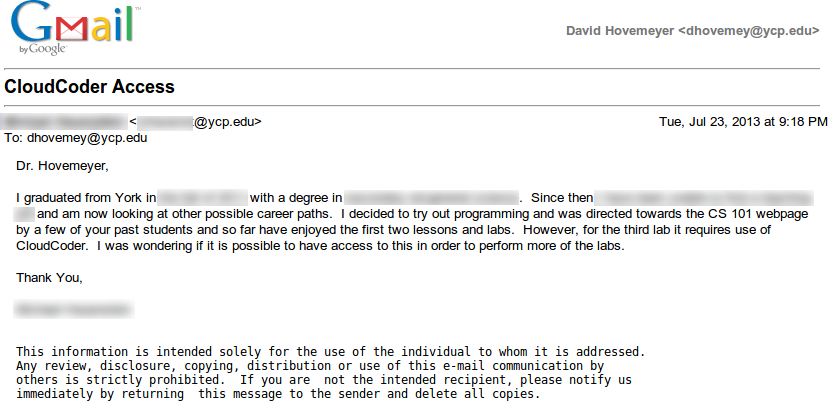
\includegraphics[width=4.5in]{images/email1}
%\end{center}
%
%[I (DH) created an account and replied with the username and password.]
%
%\end{frame}
%
%%%%%%%%%%%%%%%%%%%%%%%%% Email #2 %%%%%%%%%%%%%%%%%%%%%%%%%%%
%\begin{frame}{Email \#2}
%
%\begin{center}
%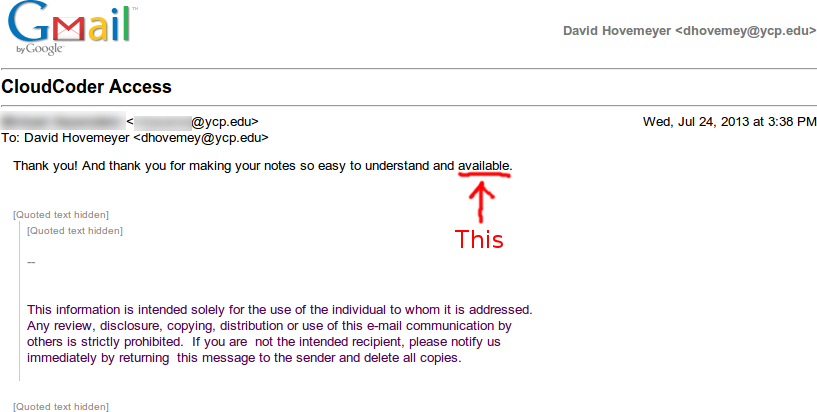
\includegraphics[width=4.5in]{images/email2}
%\end{center}
%
%\end{frame}

%%%%%%%%%%%%%%%%%%%%%%%% CloudCoder %%%%%%%%%%%%%%%%%%%%%%%%%%%
\begin{frame}{CloudCoder}

\begin{itemize}
  \item Open source (AGPL v3)
  \item Supports exercises in Java, Python, Ruby, and C/C++
  \item Collects fine-grained edit sequence of each student's work
  \item Repository of freely-redistributable (CC-BY-SA) exercises:
        \url{https://cloudcoder.org/repo}
  \item Requires two Linux servers to host (one network-facing)
    \begin{itemize}
    \item Relatively easy to install
    \item Known to support 60+ concurrent users with modest hardware
    \item Load testing experiments successful with 700+ concurrent users
          on moderate server hardware
      \begin{itemize}
      \item Compiling and testing submissions requires significant
            CPU resources, but is easy to scale up by adding more
            build servers
      \end{itemize}
    \item Cost to host per course-semester: perhaps \$1-\$3 per student
          (e.g., using Amazon EC2)
    \end{itemize}
\end{itemize}

\end{frame}

%%%%%%%%%%%%%%%%%%%%%%%% CloudCoder screenshot %%%%%%%%%%%%%%%%%%%%%%%%%%%
\begin{frame}{CloudCoder screenshot}

\begin{center}
\vskip -.15in
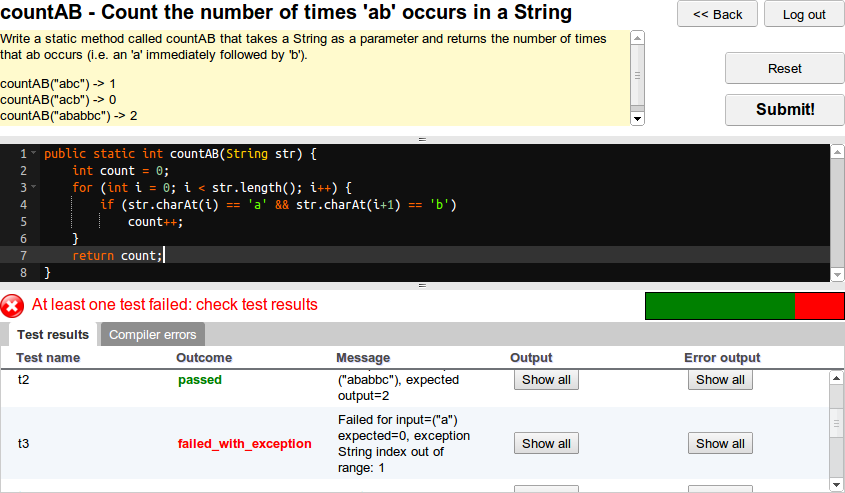
\includegraphics[width=4.5in]{images/screenshot4}
\end{center}

\end{frame}

%%%%%%%%%%%%%%%%%%%%%%%% Experiences %%%%%%%%%%%%%%%%%%%%%%%%%%%
\begin{frame}{Experiences}

\begin{itemize}
\item Pilot studies:
  \begin{itemize}
  \item Canisius College: 30 students, CS1, C++
  \item York College: 122 students, CS1, C
  \item Knox College: 23 students, CS1, Java
  \item U.\ of Auckland: 30 students, CS1, C
  \end{itemize}
\item Experiences:
  \begin{itemize}
  \item The software works, students seem to like it
  \item Writing exercises from scratch is hard
  \item Repository has 100+ exercises, but not much reuse has occurred yet
  \end{itemize}
\item Can we scale it to larger courses?
  \begin{itemize}
\item September 2013: U.\ of Auckland: 700 students, CS1, C
  \end{itemize}
\end{itemize}

\end{frame}

\end{document}
